\documentclass[letterpaper,12pt,oneside]{article}
\usepackage[top=1in, left=1.25in, right=1.25in, bottom=1in]{geometry}
\usepackage{float}
\usepackage[T1]{fontenc}
\usepackage[utf8]{inputenc}
\usepackage[english]{babel}
\usepackage{graphicx}
\usepackage{array}
\usepackage{listings}
\usepackage{hyperref}

\graphicspath{{./figs/}}

\lstset{
    basicstyle=\ttfamily\small,
    breaklines=true,
    frame=single,
    showstringspaces=false,
    captionpos=b
}

\begin{document}

%--------------------------------------------------
% PORTADA
%--------------------------------------------------

\begin{titlepage}
\setlength{\parindent}{0pt}
\setlength{\parskip}{0pt}

\begin{center}
\vfill


\includegraphics[width=4.5cm]{UNAM_LOGO2.png}

\vspace{0.5cm}
{\Huge \textbf{Universidad Nacional Autónoma de México}}

\vfill

{\large Computer Engineering}

\vfill

{\large COMPILERS}

\vspace{1cm}

{\huge PARSER \&\ SDT}

\vspace{1cm}

STUDENTS: \\
321117744 \\
321339009 \\
321008215 \\
321032308 \\
320237012 \\

\vspace{1cm}

Group: 5 \\
Team: 4 \\
Semester: 2026-II

\vfill

México, CDMX. April 30th, 2026

\end{center}
\end{titlepage}

\tableofcontents
\clearpage

%--------------------------------------------------

\section{Introduction}

\subsection{Problem Statement}
This project extends the previously developed lexical analyzer by implementing a parser and a Syntax-Directed Translation (SDT) system based on a Context-Free Grammar.

\subsection{Motivation}
To apply the concepts learned in class related to parsing techniques and semantic analysis, and to understand how different phases of a compiler interact.

\subsection{Objective}
To develop a syntactic analyzer capable of validating program structure, generating an Abstract Syntax Tree (AST), and performing semantic verification using SDT rules.

%--------------------------------------------------

\section{Theoretical Framework}

A programming language is structured through syntax and semantics.

\begin{itemize}
    \item \textbf{Syntax:} Syntax studies the way in which words are combined and what the relationships between them are to form an idea. It helps us to establish the rules that give order to a language. Also, to avoid misunderstandings and to give consistent messages [1].  
    \item \textbf{Semantics:} Semantics is the one that studies the words, signs, and the meaning of each of them [2]. [3]
\end{itemize}

Understanding language is important for the compiler, which is defined as a computer program that converts code from one programming language, to another programming language. The compiler transforms high-level language into low-level language, and it does this through a process that has the next phases: 

\begin{enumerate}
    \item Lexical analysis
    \item Syntax analysis
    \item Semantic analysis
    \item Optimization.
    \item Code generation [4]. 
\end{enumerate}

\bigskip

The lexer, a previous project, did the first analysis (lexical). The present project adds the Parser, which consists of syntax analysis, and the SDT, which extends the analysis by including semantic actions. 

\bigskip

\
A \textbf{parser} is the syntactic analysis where the computer interprets the grammatical structure of a text in language, whether it is a natural or a programming language. 

\bigskip

The \textbf{parser} breaks down words and symbols into an organized hierarchy (like a syntax tree), to identify how the elements of a sentence relate to each other according to rules established in a pre-established grammar. Depending on the order of analysis, it can be ascending \textbf{(bottom-up}) or descending (\textbf{top-down}) [5]. 

\bigskip

\textbf{SDT}, also known as "\textbf{Syntax Directed Translation}", is a technique where semantic actions are included alongside the grammar production. Allows the execution of semantic actions associated with grammar rules, enabling type checking and symbol management. [6]

\bigskip

The \textbf{AST} represents the logical structure of the program.

%--------------------------------------------------

\section{Grammar Definition}

The following Context-Free Grammar defines the structure of the Juan Pato language.

\subsection{Program Structure}

\begin{lstlisting}
program → Start { instructions }

instructions → instruction instructions
             | instruction
\end{lstlisting}

\subsection{Instructions}

\begin{lstlisting}
instruction → writing
            | reading
            | declaration
            | assignment
            | if
            | if-else
            | while
            | for
            | comment
\end{lstlisting}

\subsection{Statements}

\begin{lstlisting}
writing → printf expression ;
reading → read ID ;

declaration → TYPE ID ;
declaration → TYPE ID = expression ;

assignment → ID = expression ;
\end{lstlisting}

\subsection{Control Structures}

\begin{lstlisting}
if → if expression then { instructions }

if-else → if expression then { instructions }
          else { instructions }

while → while expression { instructions }

for → for ID from expression to expression { instructions }
\end{lstlisting}

\subsection{Expressions}

\begin{lstlisting}
expression → expression ARIT_OP expression
           | expression COMP_OP expression
           | expression BOOL_OP expression
           | ( expression )
           | ID
           | INTEGER
           | REAL
           | STRING
           | BOOL
\end{lstlisting}

%--------------------------------------------------

\section{System Design}

The compiler consists of three main modules.

%aqui no paso nada, entendido? 

\subsection{Lexical Analyzer}

The project's lexical analyzer aims to transform the input, initially represented as text, into a sequence of tokens using regular expressions, in order to prepare the information for the compiler's subsequent stages.

\bigskip

One of the libraries for implementing lexical analysis is RPLY. This is a pure Python parser generator that offers easy-to-use tools to indicate the rules needed for this type of analysis through a LexerGenerator instance, which represents a set of rules that match pieces of text that should either be turned into tokens or ignored by the Lexer. Rules are added using the method called add or ignored with 'ignore'.

\bigskip

The file called 'AnalizadorLexico.py'  is the one that carries the lexical analysis of the file, the first stage of the full compilation process. It employs the class lexer from the lexer generator library, this allows entries to be added to the lexer, by which we can define tokens with a name to identify each of them by, as well as the regular expression that the program expects to find in the .jp files and that it uses for cataloging each part of its contents. In doing so, we can define the grammar of the language for the compiler, and detect if a supposedly correct file follows the grammar properly or if it has lexical errors. It is able to classify all of the symbols and at the end of its execution, redirect the output to the main.py file to present the information to the user. 

\bigskip

Some of the tokens that it is designed to accept are: the start of a program, the brackets that limit its span, the type of a variable, a variable name, a number, an operator (arithmetic, boolean, assignation), as well as what to ignore like white spaces and comments.

\subsection{Parser}

The parser for this project was designed to validate the syntax, build an Abstract Syntax Tree (AST), and generate a symbol table from the input program. The parser is bottom up (LALR).

\bigskip

As a first step, it verifies that the tokens have the correct structure.  If there is a mistake, the parser will report us the syntax error with its line.

\bigskip

After validating the syntax, the parser builds the Abstract Syntax Tree (AST). This tree represents in a graphical and in a hierarchical way, the structure of the program. Each node in the tree is an instruction, expression, or control structure (such as if, while, or for). This helps the program to be easier to analyze.

\bigskip

Also, the parser creates a symbol table. This table shows us information about the variables used in the program, such as their type, and value. It also helps to detect cases where a variable is used without being declared.

\bigskip

There were several tests performed using different input programs.

\bigskip

One of the programs had variable declarations and arithmetic operations. When it was analyzed,the parser validated the syntax, built the AST, and stored the variables in the symbol table.

\bigskip

Other programs with control structures like \textbf{if, else}, \textbf{while}, and \textbf{for} were tested too. The parser recognized these structures and represented them correctly in the AST.

\bigskip

But in error cases where there were syntax errors or undeclared variables, the parser reported errors or warnings. This shows that the validation worked correctly.

\bigskip

Altogether, the tests showed that the parser correctly validates syntax, builds the AST, and generates the symbol table. And, when it's necessary, tell us where there is a mistake.

\subsection{Semantic Analyzer}

{The semantic analysis represents the phase where the compiler validates the logical coherence of the program. It is not enough for the code to comply with grammatical rules; the compiler functions as a filter that ensures only "perfect logic" progresses toward execution}

\bigskip

{For this purpose, the implementation of the SemAnalyzer class receives the Abstract Syntax Tree (AST) and traverses it recursively. In this process, each node of the tree is examined to guarantee that operations between variables and values are compatible, preventing underlying inconsistencies from becoming critical failures during runtime.}

\bigskip

{The operation of this analyzer depends on the Symbol Table (sym\_table), which acts as the central memory of the system by storing identifiers and their data types, whether they are integers, reals, or booleans. During the AST traversal, the tipoSubTree method consults this table every time a variable is referenced. This step is fundamental, as without such context, the analyzer has no means to verify if a variable has been previously declared or if the assigned data type corresponds to the nature of the operation. In this way, the symbol table provides real meaning to the hierarchical structure of the tree.}

\bigskip

{It is imperative to distinguish this process from syntactic analysis. While a syntax error is a failure of form, such as the omission of a semicolon that prevents the construction of the tree, a semantic error arises when the structure is valid but the instruction is logically impossible.}

\bigskip

{The analyzer is designed to detect three main categories of failures: type mismatch (such as assigning a text string to an integer variable), the use of undeclared variables, and the presence of non-boolean conditions in control structures. Detecting these failures significantly increases the robustness of the source code.}

\bigskip

{Finally, the integrity of the validation is managed through the num\_errors variable. If, upon concluding the tree review, the counter shows a value greater than zero, the compilation process is interrupted. This mechanism ensures that the user receives clear feedback on logical errors before proceeding with the execution of the software. In conclusion, the semantic analyzer verifies the coherence of the program, elevating the role of the compiler from a simple translator to a quality control tool that only allows the flow of semantically impeccable code.}

%--------------------------------------------------

\section{Results}

\subsection{Correct Program}
Parsing succeeds, AST is generated, and SDT is verified.

\begin{figure}[H]
    \centering
    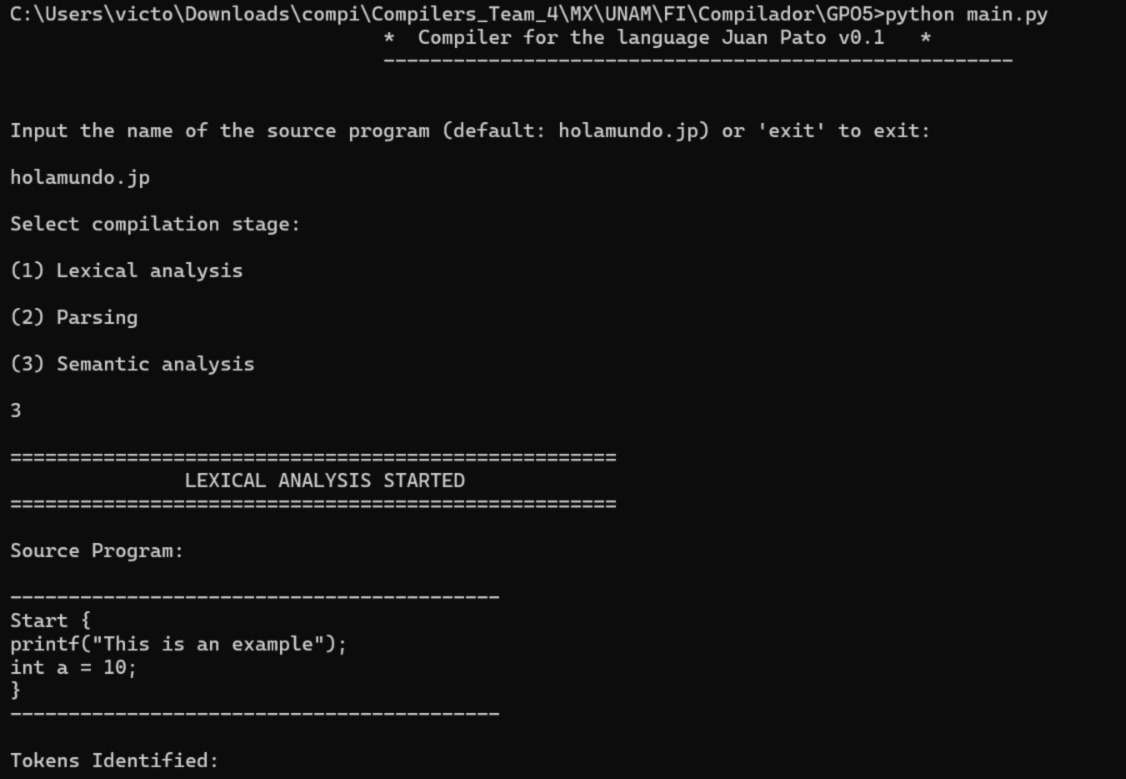
\includegraphics[width=0.5\linewidth]{CompilerHolaMundo1.jpeg}
    \caption{Analysis on a flawless file - holamundo.jp}
    \label{fig:placeholder}
\end{figure}

\begin{figure}[H]
    \centering
    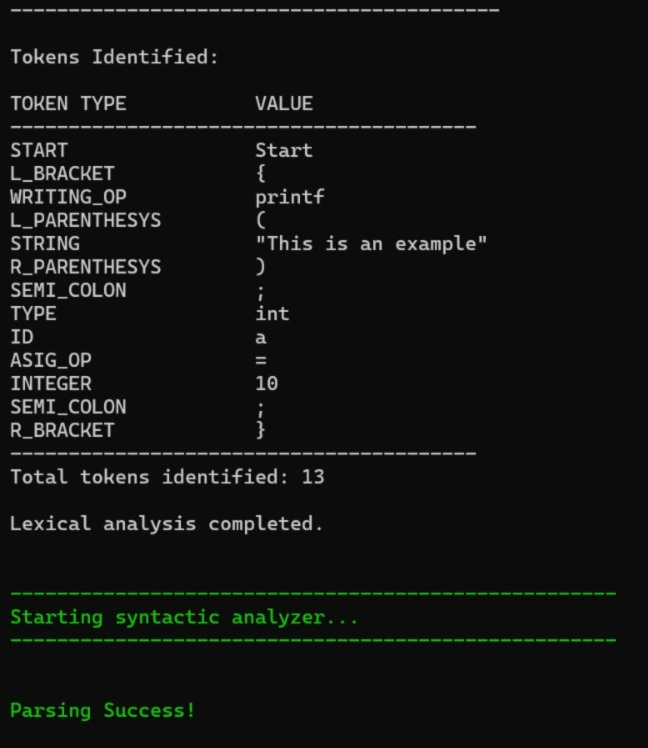
\includegraphics[width=0.5\linewidth]{CompilerHolaMundo2.jpeg}
   
    \label{fig:placeholder}
\end{figure}

\begin{figure}[H]
    \centering
    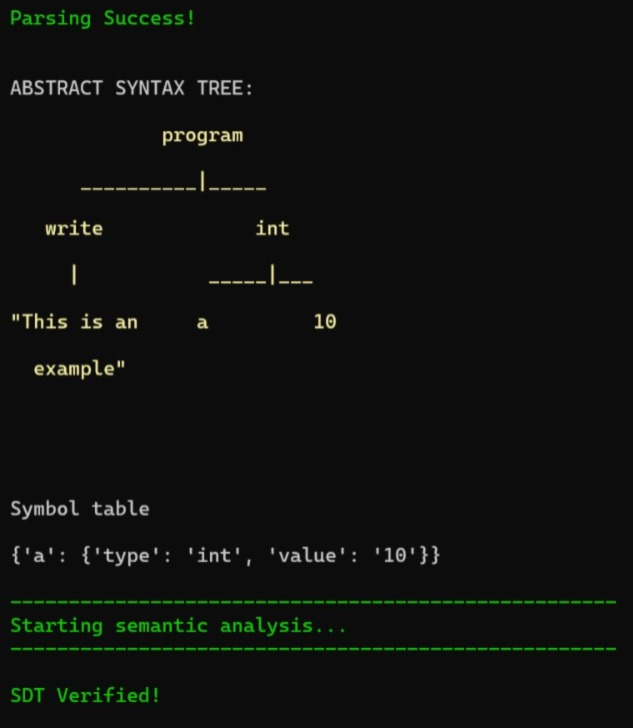
\includegraphics[width=0.5\linewidth]{CompilerHolaMundo3.jpeg}
   
    \label{fig:placeholder}
\end{figure}


\subsection{Syntax Error}
Parsing fails and semantic analysis is not executed.

\begin{figure}[H]
    \centering
    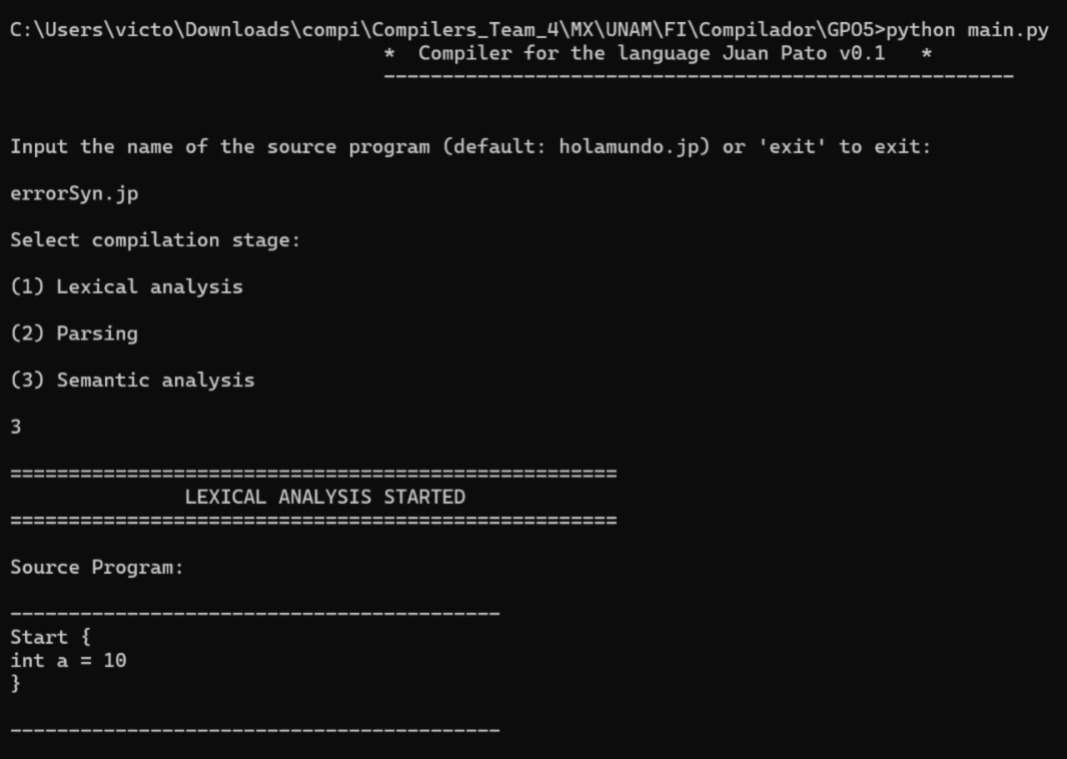
\includegraphics[width=0.5\linewidth]{CompiladorErrorSyn1.jpeg}
    \caption{Showcasing a program with syntax errors - errorSyn.jp}
    \label{fig:placeholder}
\end{figure}

\begin{figure}[H]
    \centering
    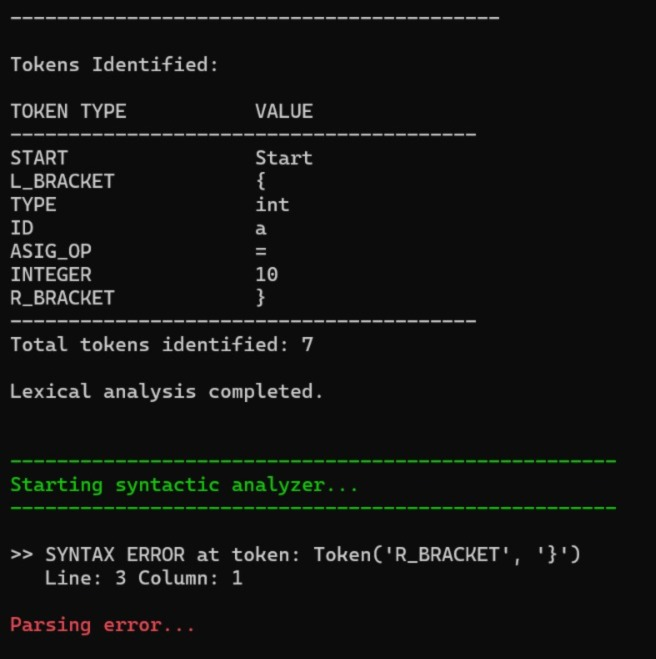
\includegraphics[width=0.5\linewidth]{CompiladorErrorSyn2.jpeg}
    \label{fig:placeholder}
\end{figure}

\subsection{Semantic Error}
Parsing succeeds but SDT reports an error.

\begin{figure}[H]
    \centering
    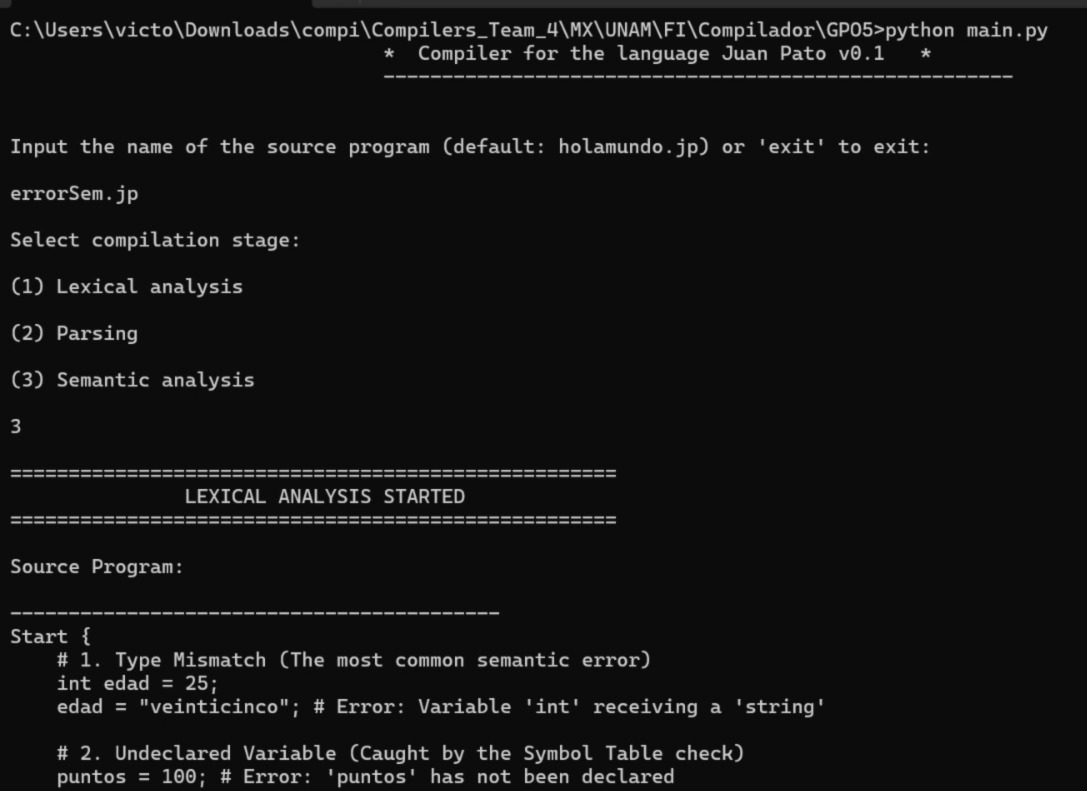
\includegraphics[width=0.5\linewidth]{CompiladorErrorSem1.jpeg}
    \caption{Showcasing a program with semantic errors - errorSem.jp}
    \label{fig:placeholder}
\end{figure}

\begin{figure}[H]
    \centering
    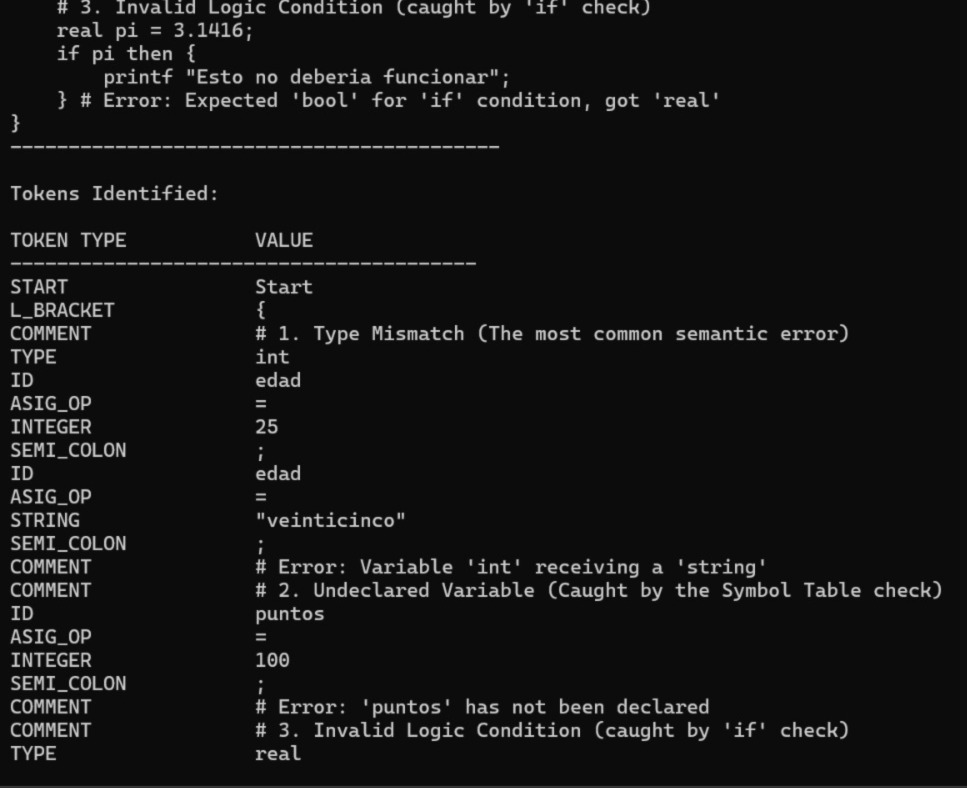
\includegraphics[width=0.5\linewidth]{CompiladorErrorSem2.jpeg}
    \label{fig:placeholder}
\end{figure}

\begin{figure}[H]
    \centering
    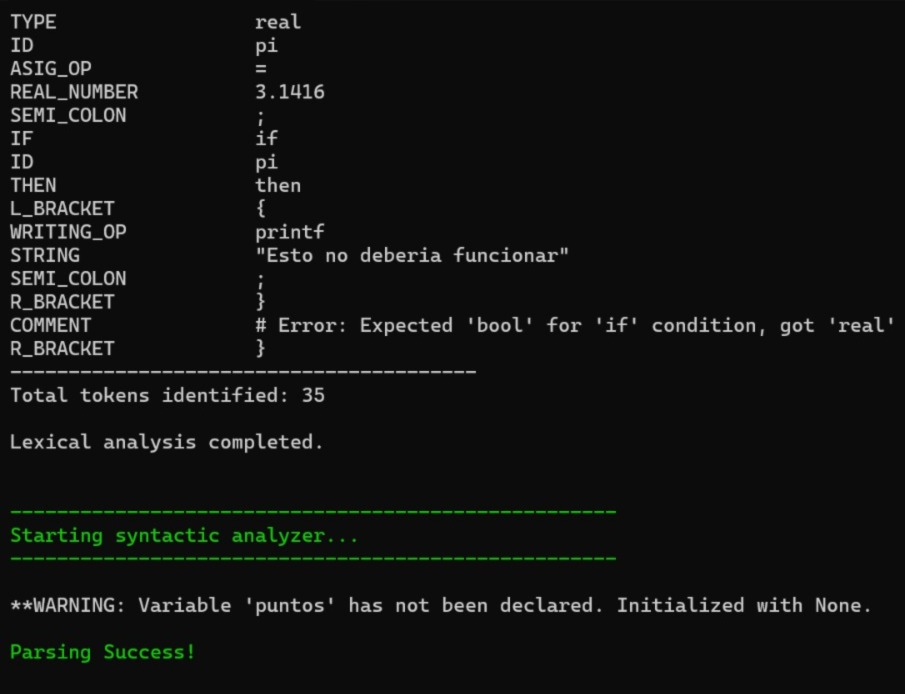
\includegraphics[width=0.5\linewidth]{CompiladorErrorSem3.jpeg}
    \label{fig:placeholder}
\end{figure}

\begin{figure}[H]
    \centering
    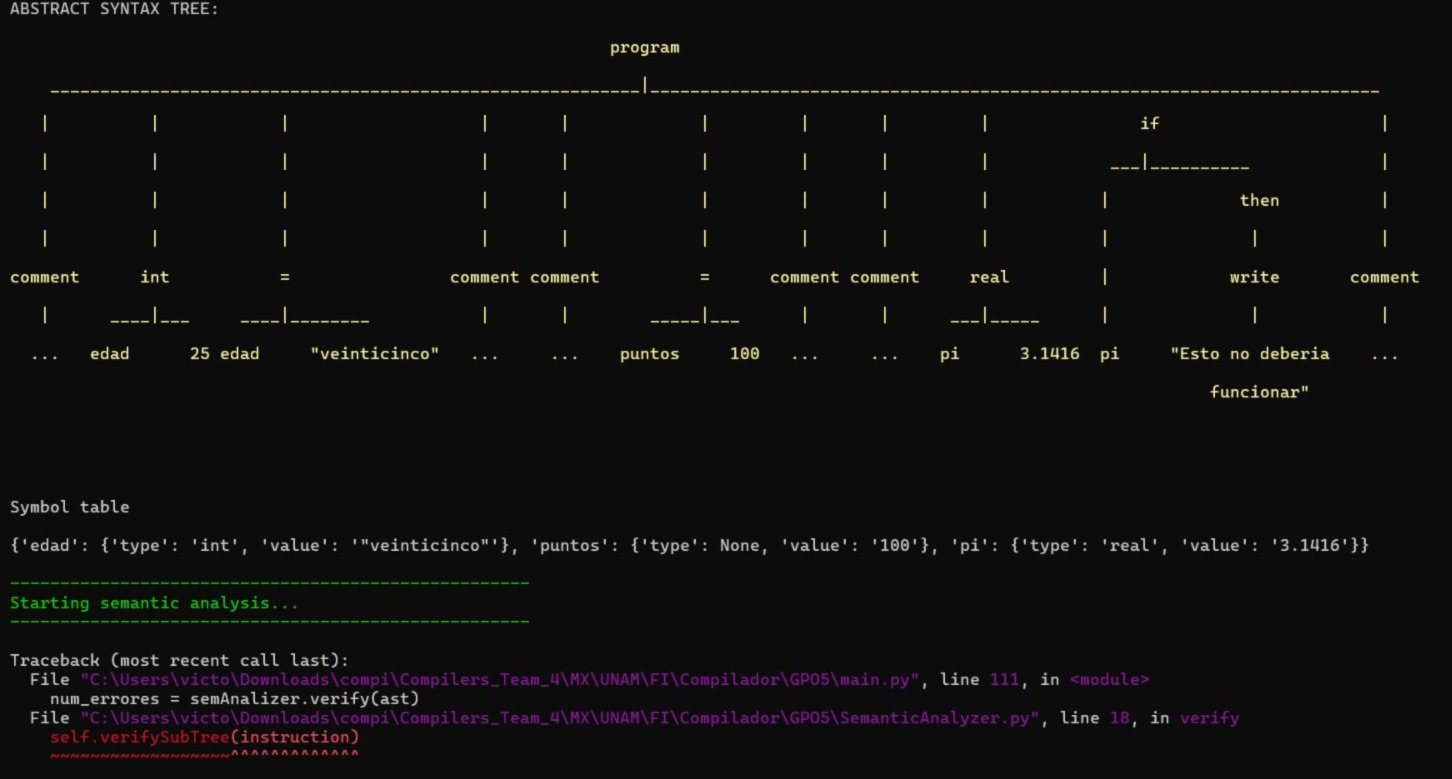
\includegraphics[width=0.5\linewidth]{CompiladorErrorSem4.jpeg}
    \label{fig:placeholder}
\end{figure}

\begin{figure}[H]
    \centering
    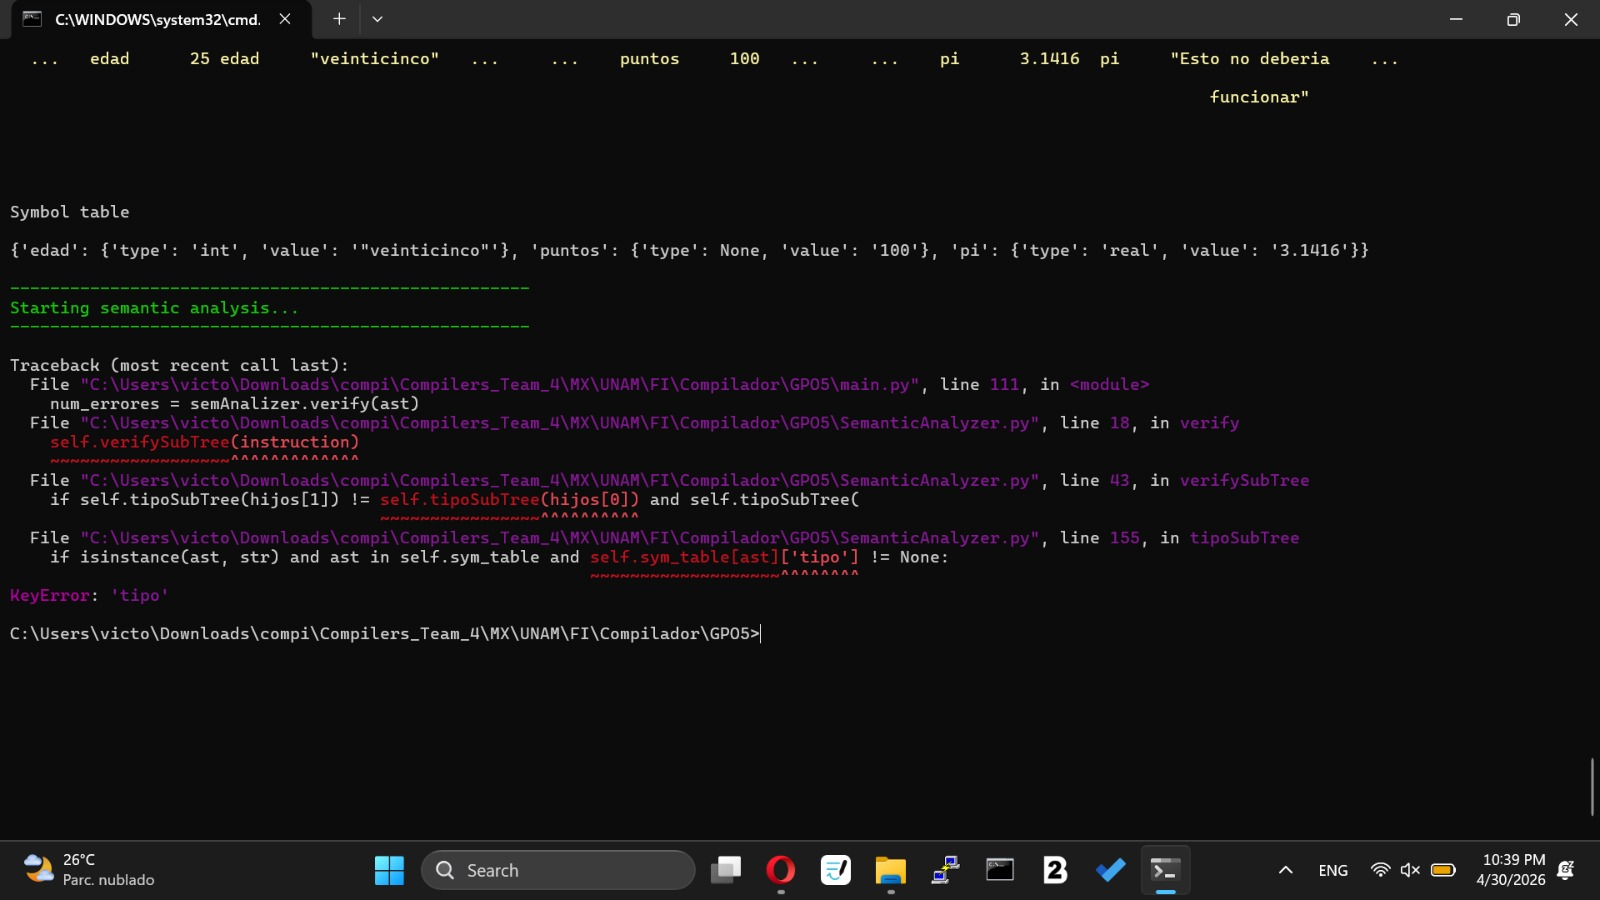
\includegraphics[width=0.5\linewidth]{CompiladorErrorSem5.jpeg}
    \label{fig:placeholder}
\end{figure}
%--------------------------------------------------

\section{Conclusions}

An analysis of the results obtained underscores the importance of applying compiler design theory to achieve consistent and reliable source code processing. The integration of lexical, syntactic, and semantic analysis demonstrates how each phase contributes to the correct interpretation of a program: from transforming plain text into structured tokens, through validating its grammatical structure, to ensuring its logical coherence. In this context, the parser and the SDT extend the compiler's functionality by validating syntax and semantics, thus ensuring the correct structure and logic of the program.

\bigskip

The results confirm that the formal definition of grammars, the use of parsing techniques such as LALR, and the implementation of semantic rules using symbol tables and tree traversal are essential for detecting inconsistencies at different levels of abstraction. This layered validation approach allows for the precise identification of errors according to their nature, reflecting the effectiveness of the theoretical foundations applied in practice.

\bigskip

Furthermore, the interaction between the Abstract Syntax Tree and the symbol table is fundamental for assigning meaning to the program beyond its structure, reinforcing the idea that compilation is not only a translation process but also a verification mechanism. Overall, the results demonstrate that the correct application of these concepts allows for the construction of a robust system capable of guaranteeing both syntactic correctness and semantic validity.

%--------------------------------------------------

\begin{thebibliography}{9}

\bibitem{islas}
B. M. Islas, 
``Sintaxis Elemental,'' 
\emph{Unidades de Apoyo para el Aprendizaje (UAPA)}, 
CUAIEED/FES Acatlán-UNAM, 
2018. 
[Online]. Available: 
\url{https://repositorio-uapa.cuaed.unam.mx/repositorio/moodle/pluginfile.php/1723/mod_resource/content/9/contenido/index.html} 
[Accessed: Apr. 29, 2026].

\bibitem{ucm}
Universidad Complutense de Madrid, 
``La semántica,'' 
\emph{Plataforma gramatical para la enseñanza del español como lengua extranjera}, 
n.d. 
[Online]. Available: 
\url{https://www.ucm.es/plataformaele/la-semantica} 
[Accessed: Apr. 29, 2026].

\bibitem{rdu}
A. Martínez Romero, J. L. Ortega Sánchez, and J. de J. Alba Romero, 
``Lenguaje: instrumento del desarrollo humano'' (English title: ``Language: instrument of human development''), 
\emph{Revista Digital Universitaria (RDU)}, 
vol. 22, no. 5, 
Sep.-Oct. 2021. 
doi: \href{https://doi.org/10.22201/cuaieed.16076079e.2021.22.5.10}{10.22201/cuaieed.16076079e.2021.22.5.10}.

\bibitem{ibm}
IBM, 
``What is a Compiler?,'' 
\emph{IBM Think}, 
n.d. 
[Online]. Available: 
\url{https://www.ibm.com/mx-es/think/topics/compiler} 
[Accessed: Apr. 29, 2026].

\bibitem{marco}
Marco, 
``Parsing,'' 
\emph{MSMK University}, 
Jul. 1, 2025. 
[Online]. Available: 
\url{https://msmk.university/parsing/} 
[Accessed: Apr. 29, 2026].

\bibitem{geeks}
GeeksforGeeks, 
``Syntax-Directed Translation Schemes,'' 
\emph{GeeksforGeeks}, 
Jul. 23, 2025. 
[Online]. Available: 
\url{https://www.geeksforgeeks.org/compiler-design/syntax-directed-translation-schemes/} 
[Accessed: Apr. 29, 2026].

\end{thebibliography}

\end{document}
